\documentclass[norsk,a4paper,12pt]{article} 
\usepackage[norsk]{babel} 
\usepackage[T1]{fontenc} %for å bruke æøå 
\usepackage[utf8x]{inputenc} 
\usepackage{graphicx} %for å inkludere grafikk 
\usepackage{verbatim} %for å inkludere filer med tegn LaTeX ikke liker 
\usepackage{amsfonts} 
\usepackage{amsmath} 
\usepackage{amssymb} 
%\usepackage{savesym} 
%\savesymbol{square} 
\bibliographystyle{plain} 
\usepackage{float} 
%\usepackage{SIunits} 
\usepackage{textcomp} 
\usepackage{parskip} 
\usepackage{array} 
%\usepackage[framed]{mcode} 
\usepackage[margin=2.3cm]{caption}
\usepackage{listings}

\begin{document}

\title{AST5220 Cosmology II: Milestone 2}
\author{Peder Forfang}
\maketitle

\section{The recombination history of the universe}
The Cosmic Microwave Background (CMB) anisotropies is an important source of information on the history of the Universe and since first discovered has been a large research field in cosmology. This report is the second part of a larger project concerning calculation of the CMB spectrum. It is a sequel to milestone 1, ``The background evolution of the universe'', where we went through calculation of the expansion history of the universe and the uniform background densities of the various matter and energy components from recombination until today. We will take a step further in this report by numerically calculating the optical depth $\tau$ of the universe back to conformal time $\eta $ and the scaled visibility function $\tilde{g}(\eta)$, which is the probability that a photon observed today was last scattered at conformal time $\eta$. The report includes one plot of $\tau(x)$, $\tau'(x)$ and $\tau''(x)$, one plot of $\tilde{g}(x)$, $\tilde{g}'(x)$ and $\tilde{g}''(x)$, as well as one plot of the fractional electron density $X_e$ as a function of redshift. We assume that the entirety of the neutral baryonic matter is in terms of hydrogen, thus $n_b \approx n_H$. 

The optical depth is a measure of how transparent our universe is. It is connected to the observed intensity $I$ of a photon with an initial intensity $I_0$ as $I = I_0e^{-\tau(\eta)}$. The current value is $\tau = 0$, thus $I = I_0$ in the universe today. The optical depth is defined as 

\begin{equation}
 \tau(\eta) = \int_{\eta}^{\eta_0} n_e\sigma_T a d\eta'
\end{equation}

where $n_e$ is the electron density, $\sigma_T $ the Thomson cross-section and $\eta_0 $ the conformal time today. More convinient numerically, the differential form of the optical depth can be written as

\begin{equation}
 \tau' = -\frac{n_e \sigma_T a}{H_p}
\end{equation}

where $H_p = aH$. We define the visibility function as

\begin{equation}
 \tilde{g}(x) = -\tau'e^{-\tau}
\end{equation}

In order to calculate these quantities, we need to find the electron density $n_e$ or rather the fractional electron density $X_e = n_e/n_H$. To do this we need to find the distribution of ionized hydrogen. As stated above, $n_H$ represents the entire baryon density. We have that

\begin{equation}
 n_H = n_b \simeq \frac{\rho_b}{m_H} = \frac{\Omega_b\rho_c}{m_Ha^3}
\end{equation}

where $\rho_c$ is the critical density today. Before recombination, $n_H$ is low and $X_e \simeq 1$. Around this time, we can approximate $X_e$ by the Saha equation, 

\begin{equation}
 \frac{X_e^2}{1 - X_e} = \frac{1}{n_b} (\frac{m_eT_b}{2\pi})^{3/2}e^{-\epsilon_0/T_b}
\end{equation}

where $T_b$ is the baryon temperature of the universe and $\epsilon_0 = 13.6$ eV is the ionization energy of hydrogen. For simplicity we have assumed $T_b$ to be equal to the radiation temperature $T_r$. This is in practice a good approximation and saves a headache. Thus we have that $T_b = T_r = T_0/a = 2.725 K/a$ and can solve the equation above as a second order equation. Later hydrogen gets neutralized, and $X_e \ll 1$. A more accurate equation is needed, so during and after recombination we will utilize the Peebles' equation,

\begin{equation}
 \frac{dX_e}{dx} = \frac{C_r(T_b)}{H}[\beta(T_b)(1-X_e) - n_H\alpha^{(2)}(T_b)X_e^2]
\end{equation}

where

\begin{equation}
 C_r(T_b) = \frac{\Lambda_{2s\rightarrow1s} + \Lambda_{\alpha}}{\Lambda_{2s\rightarrow1s} + \Lambda_{\alpha} + \beta^{(2)}(T_b)}
\end{equation}

\begin{equation}
 \Lambda_{2s\rightarrow1s} = 8.227 s^{-1}
\end{equation}

\begin{equation}
\Lambda_{\alpha} = H\frac{(3\epsilon_0)^3}{(8\pi)^2n_{1s}}
\end{equation}

\begin{equation}
 n_{1s} = (1 - X_e)n_H
\end{equation}

\begin{equation}
 \beta^{(2)} = \beta(T_b)e^{3\epsilon_0/4T_b}
\end{equation}

\begin{equation}
 \beta(T_b) = \alpha^{(2)}(T_b)(\frac{m_eT_b}{2\pi})^{3/2}e^{-\epsilon_0/T_b}
\end{equation}

\begin{equation}
 \alpha^{(2)} = \frac{64\pi}{\sqrt{27\pi}}\frac{\alpha^2}{m_e^2}\sqrt{\frac{\epsilon_0}{T_b}}\phi_2(T_b)
\end{equation}

\begin{equation}
 \phi_2(T_b) = 0.44ln(\epsilon_0/T_b)
\end{equation}

This set of constants describe the atomic physics. The equation takes into account the transition rates between the ground state (s1) and the first excited state (s2) of the hydrogen atom. In our numerical approach we will use the Saha equation when $X_e > 0.99$ and Peebles' equation when $X_e < 0.99$. Once we have computed $X_e$ we are ready to calculate the optical depth and the visibility functions.

\begin{figure}[H] 
\begin{center} 
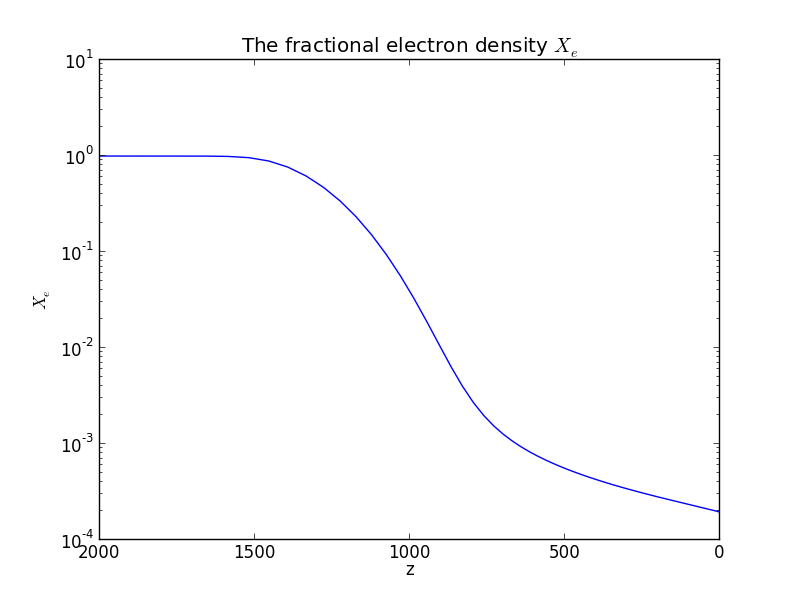
\includegraphics[scale=0.5]{Xe.png} 
 

\caption{The fractional electron density $X_e$ as a function of redshift. It rapidly decreases as recombination takes place between z = 1630.4 and z = 614.2.} 
\end{center} 
\end{figure}

\begin{figure}[H] 
\begin{center} 
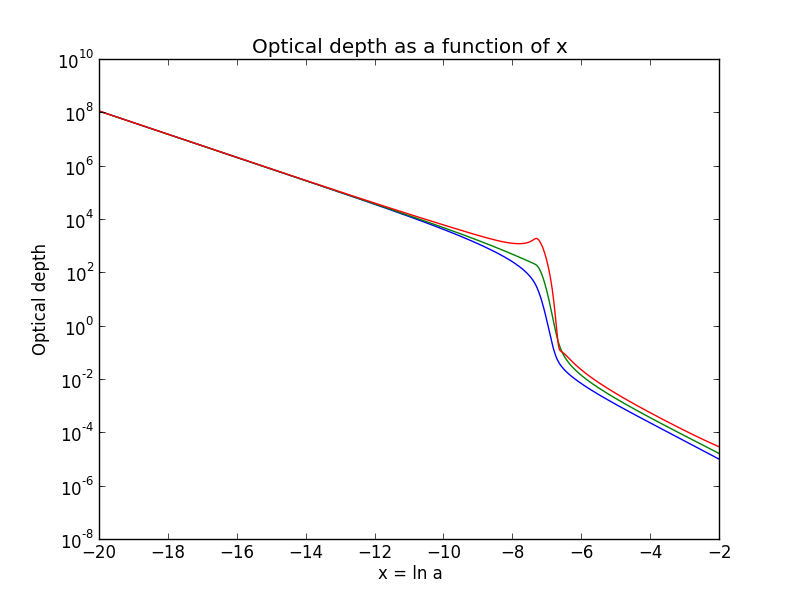
\includegraphics[scale=0.5]{tau.png} 
 

\caption{The figure shows the optical depth $\tau$ (blue line), $\tau'$ (green lime) and $\tau''$ (red line). The curves decreases fast during recombination and marks a change from an optically thick universe to an optically thin universe.} 
\end{center} 
\end{figure}


\begin{figure}[H] 
\begin{center} 
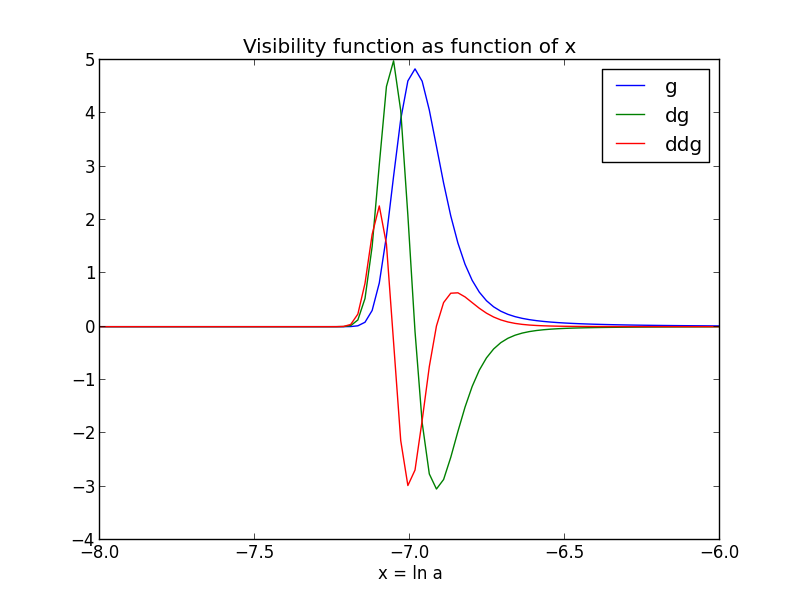
\includegraphics[scale=0.5]{g.png} 
 

\caption{The visibility function, g, and its first and second derivatives, dg and ddg, scaled to fit the same figure. The peak shows the most probable time a photon observed today was last scattered. } 
\end{center} 
\end{figure}

\end{document}
